\documentclass[12pt,t]{beamer}
\usepackage{graphicx}
\setbeameroption{hide notes}
\setbeamertemplate{note page}[plain]

% get rid of junk
\usetheme{default}
\beamertemplatenavigationsymbolsempty
\hypersetup{pdfpagemode=UseNone} % don't show bookmarks on initial view

% font
\usepackage{fontspec}
\setsansfont{TeX Gyre Heros}
\setbeamerfont{note page}{family*=pplx,size=\footnotesize} % Palatino for notes
% "TeX Gyre Heros can be used as a replacement for Helvetica"
% In Unix, unzip the following into ~/.fonts
% In Mac, unzip it, double-click the .otf files, and install using "FontBook"
%   http://www.gust.org.pl/projects/e-foundry/tex-gyre/heros/qhv2.004otf.zip

% named colors
\definecolor{offwhite}{RGB}{249,242,215}
% \definecolor{foreground}{RGB}{255,255,255}
\definecolor{foreground}{RGB}{0,0,0}
% \definecolor{background}{RGB}{24,24,24}
\definecolor{background}{RGB}{255,255,255}
\definecolor{title}{RGB}{107,174,214}
\definecolor{gray}{RGB}{100,100,100}
\definecolor{subtitle}{RGB}{102,255,204}
\definecolor{hilight}{RGB}{20,180,204}
\definecolor{vhilight}{RGB}{255,111,207}
\definecolor{lolight}{RGB}{155,155,155}
%\definecolor{green}{RGB}{125,250,125}


% use those colors
\setbeamercolor{titlelike}{fg=title}
\setbeamercolor{subtitle}{fg=subtitle}
\setbeamercolor{institute}{fg=gray}
\setbeamercolor{normal text}{fg=foreground,bg=background}
\setbeamercolor{item}{fg=foreground} % color of bullets
\setbeamercolor{subitem}{fg=gray}
\setbeamercolor{itemize/enumerate subbody}{fg=gray}
\setbeamertemplate{itemize subitem}{{\textendash}}
\setbeamerfont{itemize/enumerate subbody}{size=\footnotesize}
\setbeamerfont{itemize/enumerate subitem}{size=\footnotesize}

% page number
\setbeamertemplate{footline}{%
    \raisebox{5pt}{\makebox[\paperwidth]{\hfill\makebox[20pt]{\color{gray}
          \scriptsize\insertframenumber}}}\hspace*{5pt}}

% add a bit of space at the top of the notes page
\addtobeamertemplate{note page}{\setlength{\parskip}{12pt}}

% a few macros
\newcommand{\bi}{\begin{itemize}}
\newcommand{\ei}{\end{itemize}}
\newcommand{\ig}{\includegraphics}
\newcommand{\subt}[1]{{\footnotesize \color{subtitle} {#1}}}

% title info
\title{Data structures and stuff}
% \subtitle{Theory, Representation, and Algorithms}
\author{Gregor Behnke}
\institute{Institute of Artificial Intelligence\\ Ulm University}
\date{\tiny based on Bjarki Ágúst Guðmundsson's and Tómas Ken Magnússon's\\Competitive Programming}
% \date{\href{http://www.biostat.wisc.edu/~kbroman}{\tt \scriptsize biostat.wisc.edu/{\textasciitilde}kbroman}
% \\[-4pt]
% \href{http://github.com/kbroman}{\tt \scriptsize github.com/kbroman}
% }


\setbeamertemplate{footline}[text line]{%
  \parbox{\linewidth}{\vspace*{-8pt}Data structures and stuff \hfill \insertpagenumber}}
\setbeamertemplate{navigation symbols}{}



% Tikz
\usepackage{tikz}
\usetikzlibrary{arrows,shapes}

% Minted
\usepackage{minted}
\usemintedstyle{tango}
\newminted{cpp}{fontsize=\footnotesize}

% Graph styles
\tikzstyle{vertex}=[circle,fill=black!50,minimum size=15pt,inner sep=0pt, font=\small]
\tikzstyle{selected vertex} = [vertex, fill=red!24]
\tikzstyle{edge} = [draw,thick,-]
\tikzstyle{dedge} = [draw,thick,->]
\tikzstyle{weight} = [font=\scriptsize,pos=0.5]
\tikzstyle{selected edge} = [draw,line width=2pt,-,red!50]
\tikzstyle{ignored edge} = [draw,line width=5pt,-,black!20]


\begin{document}

% title slide
{
    \setbeamertemplate{footline}{} % no page number here
    \frame{
        \titlepage
    }
}


\begin{frame}{Today we're going to cover}
    \vspace{30pt}
    \bi
        \item Big integers
%        \item Why we need data structures
		\item \texttt{set<int>} $\approx$ \texttt{int}
        \item Augmenting binary search trees
        \item Union Find
		\item Range Query (part 1)
    \ei
\end{frame}

% \section{Big integers}
% \tableofcontents
\begin{frame}{Big integers}
    \bi
        \item What if we need to represent and do computations with very large integers, i.e.\ something that doesn't fit in a \texttt{long long}
        
        \bi
	  \item C++ has \texttt{\_\_int128\_t}
	\ei

        \vspace{5pt}
        \item Simple ideas
	  \bi
	    \item Store the integer as a string
	    \item Use Java's \texttt{BigInteger}
	  \ei
        \vspace{5pt}
        \item But how do we perform arithmetic on a pair of strings?
        \item We can use the same algorithms as we learned in elementary school
            \bi
                \item Addition: Add digit-by-digit, and maintain the carry
                \item Subtraction: Similar to addition
                \item Multiplication: Long multiplication
                \item Division: Long division
                \item Modulo: Long division
            \ei
        \item The TCR contains a C++ bigint library
    \ei
\end{frame}

\begin{frame}{Example problems}
    \bi
        \item 424 -- just implement addition or use \texttt{BigInteger}
        \item 10579 -- Fibonacci
    \ei
    
    There will be more problems in the topics ``Math'' and ``DP''
\end{frame}


\begin{frame}{Data structures you've seen before}
    \vspace{5pt}
    \bi
\item Static arrays \onslide<2->{- {\color{vhilight}int arr[10]}}
\item Dynamic arrays \onslide<2->{- {\color{vhilight}vector<int>}}
\item Linked lists \onslide<2->{- {\color{vhilight}list<int>}}
\item Stacks \onslide<2->{- {\color{vhilight}stack<int>}}
\item Queues \onslide<2->{- {\color{vhilight}queue<int>}}
\item Priority Queues \onslide<2->{- {\color{vhilight}priority\_{}queue<int>}}
\item Sets \onslide<2->{- {\color{vhilight}set<int>}}
\item Maps \onslide<2->{- {\color{vhilight}map<int, int>}}

    \onslide<3->{
        \vspace{15pt}
        \item Usually it's best to use the standard library implementations
                \bi
                    \item Almost surely bug-free and fast
                    \item We don't need to write any code
                \ei
        \item Sometimes we need our own implementation
            \bi
                \item When we want more flexibility
                \item When we want to customize the data structure
            \ei
    }
    \ei
\end{frame}


% \section{Data structures}
% \tableofcontents

\begin{frame}{Why do we need data structures?}
    \bi
        \vspace{25pt}

        \item Sometimes our data needs to be organized in a way that allows one or more of
            \bi
                \item Efficient inserting
                \item Efficient deleting
                \item Efficient querying
                \item Efficient updating
            \ei
        \item Sometimes we need a better way to represent our data
            \bi
                \item How do we represent graphs?
                \item How do we represent small sets?
                \item How do we represent \dots
            \ei

        \item Data structures help us achieve those things
    \ei
\end{frame}

%\begin{frame}{Sorting and searching}
%    \vspace{30pt}
%
%    \bi
%        \item Very common operations:
%            \bi
%                \item Sorting an array \onslide<2->{- {\color{vhilight}sort(all(arr))}}
%                \item Searching an unsorted array \onslide<2->{- {\color{vhilight}find(all(arr), x)}}
%                \item Searching a sorted array \onslide<2->{- {\color{vhilight}lower\_{}bound(all(arr), x)}}
%            \ei
%
%        \item Again, usually in the standard library
%        \item We'll need different versions of binary search later which need custom code, but lower\_{}bound is enough for now
%		    \ei
%\end{frame}
%
%\begin{frame}{Applications of Arrays and Linked Lists}
%    \vspace{40pt}
%    \bi
%        \item Too many to list
%        \item Most problems require storing data, usually in an array
%    \ei
%\end{frame}
%
%\begin{frame}{Example problem: Broken Keyboard}
%    \bi
%        \item http://uva.onlinejudge.org/external/119/11988.html
%    \ei
%\end{frame}
%
%\begin{frame}{Applications of Stacks}
%    \bi
%        \item Processing events in a first-in first-out order
%        \item Simulating recursion
%        \item Depth-first search in a graph
%        \item Reverse a sequence
%        \item Matching brackets
%        \item And a lot more
%    \ei
%\end{frame}
%
%\begin{frame}{Applications of Queues}
%    \bi
%        \item Processing events in a first-in first-out order
%        \item Breadth-first search in a graph
%        \item And a lot more
%    \ei
%\end{frame}
%
%\begin{frame}{Applications of Priority Queues}
%    \bi
%        \item Processing events in order of priority
%        \item Finding a shortest path in a graph
%        \item Some greedy algorithms
%        \item And a lot more
%    \ei
%\end{frame}
%
%\begin{frame}{Applications of Sets}
%    \bi
%        \item Keep track of distinct items
%        \item Have we seen an item before?
%        \item If implemented as a binary search tree:
%            \bi
%        \item Find the successor of an element (the smallest element that is greater than the given element)
%        \item Count how many elements are less than a given element
%        \item Count how many elements are between two given elements
%        \item Find the $k$th largest element
%            \ei
%
%        \item And a lot more
%    \ei
%\end{frame}
%
%\begin{frame}{Applications of Maps}
%    \bi
%        \item Associating a value with a key
%        \item As a frequency table
%        \item As a memory when we're doing Dynamic Programming (later)
%        \item And a lot more
%    \ei
%\end{frame}



\begin{frame}[fragile]{Representing sets}
    \vspace{30pt}
    \bi
        \item We have a small ($n\leq 30$) number of items
        \item We label them with integers in the range $0,1,\ldots,n-1$
        \item We can represent sets of these items as a 32-bit integer
        \item The $i$th item is in the set represented by the integer $x$ if the $i$th bit in $x$ is $1$
        \item Example:
            \bi
                \item We have the set $\{0,3,4\}$
                \item \mint{cpp}.int x = (1<<0) | (1<<3) | (1<<4);.
            \ei
    \ei
\end{frame}

\begin{frame}[fragile]{Representing sets}
    \vspace{5pt}
    \bi
        \item Empty set:
            \mint{cpp}.   0.
        \item Single element set:
            \mint{cpp}.   1<<i.
        \item The universe set (i.e.\ all elements):
            \mint{cpp}.   (1<<n)-1.
        \item Union of sets:
            \mint{cpp}.   x|y.
        \item Intersection of sets: \mint{cpp}.   x&y.
        \item Complement of a set: \mint{cpp}.   ~x & ((1<<n)-1).
    \ei
\end{frame}


\begin{frame}[fragile]{Representing sets}
    \vspace{25pt}
    \bi
        \item Check if an element is in the set:
            \begin{minted}{cpp}

if (x & (1<<i)) {
    // yes
} else {
    // no
}
            \end{minted}
    \ei
\end{frame}

\begin{frame}{Representing sets}
    \vspace{25pt}
    \bi
        \item Why do this instead of using {\color{vhilight}set<int>}?
        \item Very lightweight representation
        \item All subsets of the $n$ elements can be represented by integers in the range $0\ldots 2^{n}-1$
        \item Allows for easily iterating through all subsets (we'll see this later)
        \item Allows for easily using a set as an index of an array (we'll see this later)
    \ei
\end{frame}


\begin{frame}{Augmenting Data Structures}
    \bi
        \item Sometimes we can store extra information in our data structures to gain more functionality
        \item Usually we can't do this to data structures in the standard library
        \item Need our own implementation that we can customize
        \item Example: Augmenting binary search trees
    \ei
\end{frame}

\begin{frame}[fragile]{Augmenting Binary Search Trees}

    \begin{columns}[T]
        \begin{column}{.45\textwidth}
            \vspace{20pt}

            \bi
                \item We have a binary search tree and want to efficiently:
                    \bi
                        \item Count number of elements $<x$
                        \item Find the $k$th smallest element
                    \ei

                \item Naive method is to go through all vertices, but that is slow: $O(n)$
            \ei
        \end{column}%
        \hfill%
        \begin{column}{.55\textwidth}
            \begin{figure}
\tikzset{
  treenode/.style = {align=center, inner sep=0pt, text centered,
    font=\sffamily},
  vertex/.style = {treenode, circle, black, font=\sffamily\bfseries\tiny, draw=black,
    text width=1.8em},% arbre rouge noir, noeud noir
}

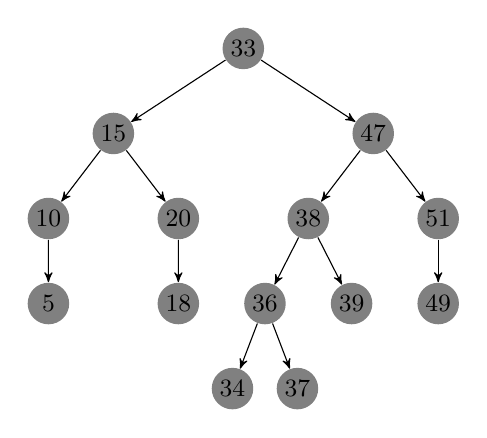
\begin{tikzpicture}[->,>=stealth',level/.style={sibling distance = 5.5cm/#1,
  level distance = 1.8cm},scale=0.6] 
\node [vertex] {33}
    child{ node [vertex] {15}
            child{ node [vertex] {10} 
            	child{ node [vertex] {5} } %for a named pointer
                % child{ node [vertex] {}}
            }
            child{ node [vertex] {20}
							child{ node [vertex] {18}}
							% child{ node [vertex] {}}
            }                            
    }
    child{ node [vertex] {47}
            child{ node [vertex] {38} 
							child{ node [vertex] {36}
                                child { node [vertex] {34} }
                                child { node [vertex] {37} }
                            }
							child{ node [vertex] {39}}
            }
            child{ node [vertex] {51}
							child{ node [vertex] {49}}
							% child{ node [vertex] {}}
            }
		}
; 
\end{tikzpicture}
            \end{figure}
        \end{column}%
    \end{columns}
\end{frame}

\begin{frame}[fragile]{Augmenting Binary Search Trees}

    \begin{columns}[T]
        \begin{column}{.45\textwidth}
            \vspace{20pt}

            \bi
                \item Idea: In each vertex store the size of the subtree
                \item This information can be maintained when we insert/delete elements without adding time complexity
            \ei
        \end{column}%
        \hfill%
        \begin{column}{.55\textwidth}
            \begin{figure}
\tikzset{
  treenode/.style = {align=center, inner sep=0pt, text centered,
    font=\sffamily},
   vertex/.style = {treenode, circle, black, font=\sffamily\bfseries\tiny, draw=black,
    text width=1.8em},% arbre rouge noir, noeud noir
}

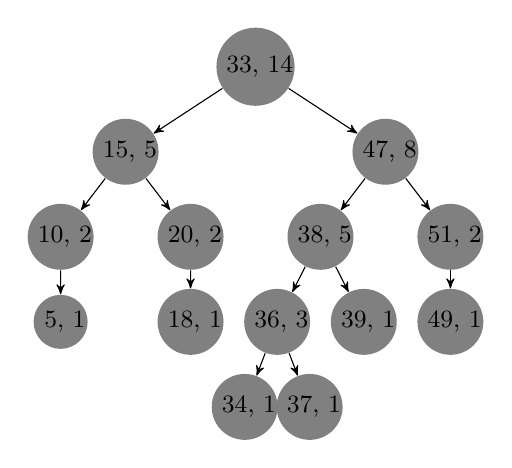
\begin{tikzpicture}[->,>=stealth',level/.style={sibling distance = 5.5cm/#1,
  level distance = 1.8cm},scale=0.6] 
\node [vertex] {\mbox{\ 33, 14}}
    child{ node [vertex] {\mbox{\ 15, 5}}
            child{ node [vertex] {\mbox{\ 10, 2}} 
            	child{ node [vertex] {\mbox{\ 5, 1}} } %for a named pointer
                % child{ node [vertex] {}}
            }
            child{ node [vertex] {\mbox{\ 20, 2}}
							child{ node [vertex] {\mbox{\ 18, 1}}}
							% child{ node [vertex] {}}
            }                            
    }
    child{ node [vertex] {\mbox{\ 47, 8}}
            child{ node [vertex] {\mbox{\ 38, 5} }
                            child{ node [vertex] {\mbox{\ 36, 3}}
                                child { node [vertex] {\mbox{\ 34, 1}} }
                                child { node [vertex] {\mbox{\ 37, 1}} }
                            }
							child{ node [vertex] {\mbox{\ 39, 1}}}
            }
            child{ node [vertex] {\mbox{\ 51, 2}}
							child{ node [vertex] {\mbox{\ 49, 1}}}
							% child{ node [vertex] {}}
            }
		}
; 
\end{tikzpicture}
            \end{figure}
        \end{column}%
    \end{columns}
\end{frame}

\begin{frame}[fragile]{Augmenting Binary Search Trees}

    \begin{columns}[T]
        \begin{column}{.45\textwidth}
            \bi
                \item Count number of elements $<38$
                    \bi
                        \item Search for $38$ in the tree
                        \item Count the vertices that we pass by that are less than $x$
                        \item When we are at a vertex where we should go right, get the size of the left subtree and add it to our count
                    \ei
            \ei
        \end{column}%
        \hfill%
        \begin{column}{.55\textwidth}
            \begin{figure}
\tikzset{
  treenode/.style = {align=center, inner sep=0pt, text centered,
    font=\sffamily},
   vertex/.style = {treenode, circle, black, font=\sffamily\bfseries\tiny, draw=black,
    text width=1.8em},% arbre rouge noir, noeud noir
}

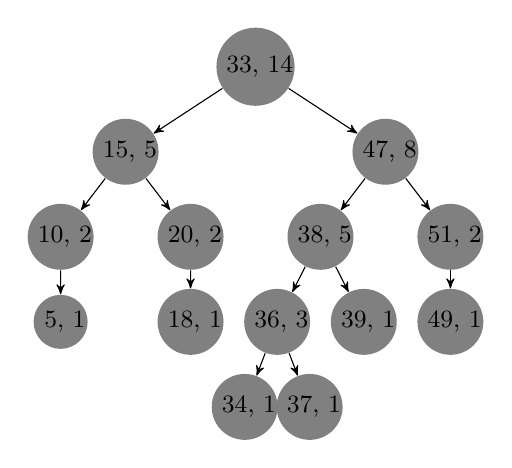
\begin{tikzpicture}[->,>=stealth',level/.style={sibling distance = 5.5cm/#1,
  level distance = 1.8cm},scale=0.6] 
\node [vertex] {\mbox{\ 33, 14}}
    child{ node [vertex] {\mbox{\ 15, 5}}
            child{ node [vertex] {\mbox{\ 10, 2}} 
            	child{ node [vertex] {\mbox{\ 5, 1}} } %for a named pointer
                % child{ node [vertex] {}}
            }
            child{ node [vertex] {\mbox{\ 20, 2}}
							child{ node [vertex] {\mbox{\ 18, 1}}}
							% child{ node [vertex] {}}
            }                            
    }
    child{ node [vertex] {\mbox{\ 47, 8}}
            child{ node [vertex] {\mbox{\ 38, 5} }
                            child{ node [vertex] {\mbox{\ 36, 3}}
                                child { node [vertex] {\mbox{\ 34, 1}} }
                                child { node [vertex] {\mbox{\ 37, 1}} }
                            }
							child{ node [vertex] {\mbox{\ 39, 1}}}
            }
            child{ node [vertex] {\mbox{\ 51, 2}}
							child{ node [vertex] {\mbox{\ 49, 1}}}
							% child{ node [vertex] {}}
            }
		}
; 
\end{tikzpicture}
            \end{figure}
        \end{column}%
    \end{columns}
\end{frame}

\begin{frame}[fragile]{Augmenting Binary Search Trees}

    \begin{columns}[T]
        \begin{column}{.45\textwidth}
            \bi
                \item Count number of elements $<38$
                    \bi
                        \item Search for $38$ in the tree
                        \item Count the vertices that we pass by that are less than $x$
                        \item When we are at a vertex where we should go right, get the size of the left subtree and add it to our count
                    \ei
                \vspace{2pt}
                \item Time complexity $O(\log n)$
            \ei
        \end{column}%
        \hfill%
        \begin{column}{.55\textwidth}
            \begin{figure}
\tikzset{
  treenode/.style = {align=center, inner sep=0pt, text centered,
    font=\sffamily},
  vertex/.style = {treenode, circle, black, font=\sffamily\bfseries\tiny, draw=black, text width=1.8em},% arbre rouge noir, noeud noir
  rvertex/.style = {treenode, circle, black, font=\sffamily\bfseries\tiny, draw=red, text width=1.8em},% arbre rouge noir, noeud noir
}

\begin{tikzpicture}[->,>=stealth',level/.style={sibling distance = 5.5cm/#1,
  level distance = 1.8cm},scale=0.6] 
\node [rvertex] {\mbox{\ 33, 14}}
    child{ node [vertex] {\mbox{\ 15, {\color{red}5}}}
            child{ node [vertex] {\mbox{\ 10, 2}} 
            	child{ node [vertex] {\mbox{\ 5, 1}} } %for a named pointer
                % child{ node [vertex] {}}
            }
            child{ node [vertex] {\mbox{\ 20, 2}}
							child{ node [vertex] {\mbox{\ 18, 1}}}
							% child{ node [vertex] {}}
            }                            
    }
    child{ node [rvertex] {\mbox{\ 47, 8}}
            child{ node [rvertex] {\mbox{\ 38, 5} }
                            child{ node [vertex] {\mbox{\ 36, {\color{red}3}}}
                                child { node [vertex] {\mbox{\ 34, 1}} }
                                child { node [vertex] {\mbox{\ 37, 1}} }
                            }
							child{ node [vertex] {\mbox{\ 39, 1}}}
            }
            child{ node [vertex] {\mbox{\ 51, 2}}
							child{ node [vertex] {\mbox{\ 49, 1}}}
							% child{ node [vertex] {}}
            }
		}
; 
\end{tikzpicture}
            \end{figure}
        \end{column}%
    \end{columns}
\end{frame}

\begin{frame}[fragile]{Augmenting Binary Search Trees}

    \begin{columns}[T]
        \begin{column}{.45\textwidth}
            \bi
                \item Find $k$th smallest element
                    \bi
                        \item We're on a vertex whose left subtree is of size $m$
                        \item If $k = m+1$, we found it
                        \item If $k \leq m$, look for the $k$th smallest element in the left subtree
                        \item If $k > m+1$, look for the $k-m-1$st smallest element in the right subtree
                    \ei
                \vspace{2pt}
            \ei
        \end{column}%
        \hfill%
        \begin{column}{.55\textwidth}
            \begin{figure}
\tikzset{
  treenode/.style = {align=center, inner sep=0pt, text centered,
    font=\sffamily},
  vertex/.style = {treenode, circle, black, font=\sffamily\bfseries\tiny, draw=black, text width=1.8em},% arbre rouge noir, noeud noir
  rvertex/.style = {treenode, circle, black, font=\sffamily\bfseries\tiny, draw=red, text width=1.8em},% arbre rouge noir, noeud noir
}

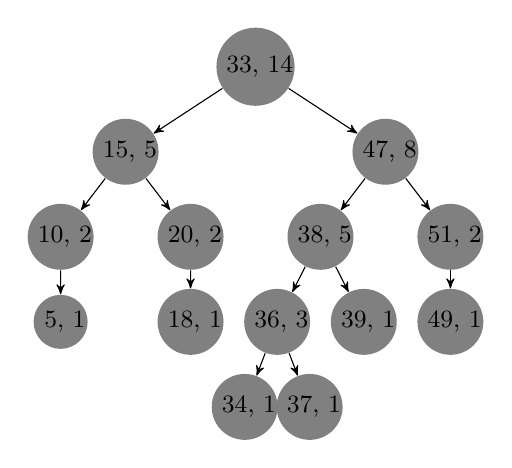
\begin{tikzpicture}[->,>=stealth',level/.style={sibling distance = 5.5cm/#1,
  level distance = 1.8cm},scale=0.6] 
\node [vertex] {\mbox{\ 33, 14}}
    child{ node [vertex] {\mbox{\ 15, 5}}
            child{ node [vertex] {\mbox{\ 10, 2}} 
            	child{ node [vertex] {\mbox{\ 5, 1}} } %for a named pointer
                % child{ node [vertex] {}}
            }
            child{ node [vertex] {\mbox{\ 20, 2}}
							child{ node [vertex] {\mbox{\ 18, 1}}}
							% child{ node [vertex] {}}
            }                            
    }
    child{ node [vertex] {\mbox{\ 47, 8}}
            child{ node [vertex] {\mbox{\ 38, 5} }
                            child{ node [vertex] {\mbox{\ 36, 3}}
                                child { node [vertex] {\mbox{\ 34, 1}} }
                                child { node [vertex] {\mbox{\ 37, 1}} }
                            }
							child{ node [vertex] {\mbox{\ 39, 1}}}
            }
            child{ node [vertex] {\mbox{\ 51, 2}}
							child{ node [vertex] {\mbox{\ 49, 1}}}
							% child{ node [vertex] {}}
            }
		}
; 
\end{tikzpicture}
            \end{figure}
        \end{column}%
    \end{columns}
\end{frame}

\begin{frame}[fragile]{Augmenting Binary Search Trees}

    \begin{columns}[T]
        \begin{column}{.45\textwidth}
            \bi
                \item Find $k$th smallest element
                    \bi
                        \item We're on a vertex whose left subtree is of size $m$
                        \item If $k = m+1$, we found it
                        \item If $k \leq m$, look for the $k$th smallest element in the left subtree
                        \item If $k > m+1$, look for the $k-m-1$st smallest element in the right subtree
                    \ei
                \item Example: $k=11$
            \ei
        \end{column}%
        \hfill%
        \begin{column}{.55\textwidth}
            \begin{figure}
\tikzset{
  treenode/.style = {align=center, inner sep=0pt, text centered,
    font=\sffamily},
  vertex/.style = {treenode, circle, black, font=\sffamily\bfseries\tiny, draw=black, text width=1.8em},% arbre rouge noir, noeud noir
  rvertex/.style = {treenode, circle, black, font=\sffamily\bfseries\tiny, draw=red, text width=1.8em},% arbre rouge noir, noeud noir
}

\begin{tikzpicture}[->,>=stealth',level/.style={sibling distance = 5.5cm/#1,
  level distance = 1.8cm},scale=0.6] 
\node [rvertex] {\mbox{\ 33, 14}}
    child{ node [vertex] {\mbox{\ 15, 5}}
            child{ node [vertex] {\mbox{\ 10, 2}} 
            	child{ node [vertex] {\mbox{\ 5, 1}} } %for a named pointer
                % child{ node [vertex] {}}
            }
            child{ node [vertex] {\mbox{\ 20, 2}}
							child{ node [vertex] {\mbox{\ 18, 1}}}
							% child{ node [vertex] {}}
            }                            
    }
    child{ node [rvertex] {\mbox{\ 47, 8}}
            child{ node [rvertex] {\mbox{\ 38, 5} }
                            child{ node [vertex] {\mbox{\ 36, 3}}
                                child { node [vertex] {\mbox{\ 34, 1}} }
                                child { node [vertex] {\mbox{\ 37, 1}} }
                            }
							child{ node [rvertex] {\mbox{\ 39, 1}}}
            }
            child{ node [vertex] {\mbox{\ 51, 2}}
							child{ node [vertex] {\mbox{\ 49, 1}}}
							% child{ node [vertex] {}}
            }
		}
; 
\end{tikzpicture}
            \end{figure}
        \end{column}%
    \end{columns}
\end{frame}

\begin{frame}[fragile]{Example}

    \bi
      \item 11991 - only construct the tree
      \item 10909 - remove elements
    \ei
\end{frame}


% TODO: Union-Find
\begin{frame}[fragile]{Union-Find}
    \vspace{20pt}
    \bi
        \item We have $n$ items
        \item Maintains a collection of disjoint sets
        \item Each of the $n$ items is in exactly one set
        \vspace{10pt}
        \item $items = \{1,2,3,4,5,6\}$
        \item $collections = \{1,4\}, \{3,5,6\}, \{2\}$
        \item $collections = \{1\}, \{2\}, \{3\}, \{4\}, \{5\}, \{6\}$
        \vspace{10pt}
        \item Supports two operations efficiently: \texttt{find(x)} and \texttt{union(x,y)}.
    \ei
\end{frame}

\begin{frame}{Union-Find}
    \bi
        \vspace{10pt}
        \item $items = \{1,2,3,4,5,6\}$
        \item $collections = \{1,4\}, \{3,5,6\}, \{2\}$
        \vspace{10pt}
        \item \texttt{find(x)} returns a representative item from the set that $x$ is in
            \bi
                \vspace{5pt}
                \item \texttt{find(1) = 1}
                \item \texttt{find(4) = 1}
                \vspace{5pt}
                \item \texttt{find(3) = 5}
                \item \texttt{find(5) = 5}
                \item \texttt{find(6) = 5}
                \vspace{5pt}
                \item \texttt{find(2) = 2}
            \ei
        \vspace{5pt}
        \item $a$ and $b$ are in the same set if and only if \\ \texttt{find(a) == find(b)}
    \ei
\end{frame}

\begin{frame}{Union-Find}
    \bi
        \vspace{10pt}
        \item $items = \{1,2,3,4,5,6\}$
        \item $collections = \{1,4\}, \{3,5,6\}, \{2\}$
        \vspace{10pt}
        \item \texttt{union(x, y)} merges the set containing $x$ and the set containing $y$ together.
        \vspace{10pt}
            \bi
                \item \texttt{union(4, 2)}
                \item $collections = \{1,2,4\}, \{3,5,6\}$
                \item \texttt{union(3, 6)}
                \item $collections = \{1,2,4\}, \{3,5,6\}$
                \item \texttt{union(2, 6)}
                \item $collections = \{1,2,3,4,5,6\}$
            \ei
    \ei
\end{frame}

\begin{frame}[fragile]{Union-Find implementation}
    \bi
        \item Quick Union with path compression
        \item Extremely simple implementation
        \item Extremely efficient
    \ei

    \vspace{10pt}

    \begin{minted}{cpp}
int pa[MAXN];
int rk[MAXN];

int ufind(int i) {
    if(pa[i]!=i) pa[i]=ufind(pa[i]);
    return pa[i];
}
    \end{minted}
\end{frame}

\begin{frame}[fragile]{Union-Find implementation}

    \begin{minted}{cpp}
int pa[MAXN];
int rk[MAXN];

int uunion(int a,int b) {
    a=ufind(a);
    b=ufind(b);
    if(a == b) return 0;
    if(rk[a]>rk[b])
        pa[b]=a;
    else
        pa[a]=b;
    if(rk[a]==rk[b]) rk[b]++;
    return 1;
}
    \end{minted}
\end{frame}

\begin{frame}[fragile]{Union-Find implementation (short)}
    \bi
        \item If you're in a hurry...
    \ei

\vspace{20pt}

    \begin{minted}{cpp}
#define MAXN 1000
int p[MAXN];

int find(int x) {
    return p[x] == x ? x : p[x] = find(p[x]); }
void unite(int x, int y) { p[find(x)] = find(y); }

FOR(i,0,n) p[i] = i;
    \end{minted}
\end{frame}

\begin{frame}{Union-Find applications}
    \vspace{30pt}
    \bi
        \item Union-Find maintains a collection of disjoint sets
        \item When are we dealing with such collections?
        \item Most common example is in graphs
    \ei
\end{frame}

\begin{frame}{Disjoint sets in graphs}
    \begin{figure}
        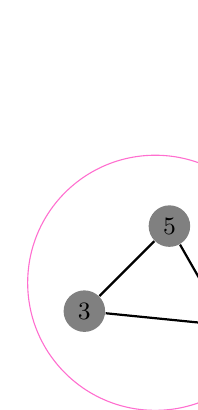
\begin{tikzpicture}[scale=1.8,auto,swap]

            \node[vertex] (1) at (-0.8,1.9) {1};
            \node[vertex] (2) at (3,1.7) {2};
            \node[vertex] (3) at (0.4,0.5) {3};
            \node[vertex] (4) at (-1.2,1.2) {4};
            \node[vertex] (5) at (1,1.1) {5};
            \node[vertex] (6) at (1.4,0.4) {6};
            \node[vertex] (7) at (-1.9,1.7) {7};

            \path[edge] (1) -- (4);
            \path[edge] (4) -- (7);
            \path[edge] (3) -- (5);
            \path[edge] (5) -- (6);
            \path[edge] (6) -- (3);

            \onslide<3->{
                \draw[color=vhilight] (-1.3,1.55) ellipse (0.9cm and 0.9cm);
                \draw[color=vhilight] (0.9,0.7) ellipse (0.9cm and 0.9cm);
                \draw[color=vhilight] (3,1.7) ellipse (0.3cm and 0.3cm);
            }

            \pgfresetboundingbox
            \path [use as bounding box] (0,0) rectangle (1,2.5);
        \end{tikzpicture}
    \end{figure}

    \bi
        \onslide<2->{\item $items = \{1,2,3,4,5,6,7\}$}
        \onslide<3->{\item $collections = \{1,4,7\}, \{2\}, \{3,5,6\}$}
        \onslide<4->{\item \texttt{union(2, 5)}}
    \ei
\end{frame}


\begin{frame}{Disjoint sets in graphs}
    \begin{figure}
        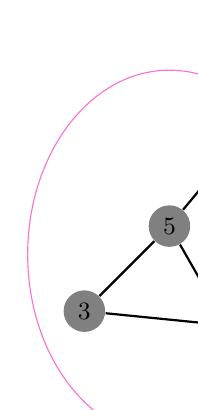
\begin{tikzpicture}[scale=1.8,auto,swap]

            \node[vertex] (1) at (-0.8,1.9) {1};
            \node[vertex] (2) at (1.5,1.7) {2};
            \node[vertex] (3) at (0.4,0.5) {3};
            \node[vertex] (4) at (-1.2,1.2) {4};
            \node[vertex] (5) at (1,1.1) {5};
            \node[vertex] (6) at (1.4,0.4) {6};
            \node[vertex] (7) at (-1.9,1.7) {7};

            \path[edge] (1) -- (4);
            \path[edge] (4) -- (7);
            \path[edge] (3) -- (5);
            \path[edge] (5) -- (6);
            \path[edge] (6) -- (3);
            \path[edge] (2) -- (5);

            \draw[color=vhilight] (-1.3,1.55) ellipse (0.9cm and 0.9cm);
            \draw[color=vhilight] (1.0,0.9) ellipse (1.0cm and 1.3cm);

            \pgfresetboundingbox
            \path [use as bounding box] (0,0) rectangle (1,2.5);
        \end{tikzpicture}
    \end{figure}

    \bi
        \item $items = \{1,2,3,4,5,6,7\}$
        \item $collections = \{1,4,7\}, \{2,3,5,6\}$
        \onslide<2->{\item \texttt{union(6, 2)}}
    \ei
\end{frame}


\begin{frame}{Disjoint sets in graphs}
    \begin{figure}
        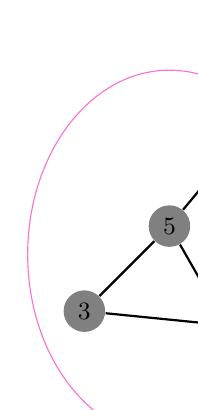
\begin{tikzpicture}[scale=1.8,auto,swap]

            \node[vertex] (1) at (-0.8,1.9) {1};
            \node[vertex] (2) at (1.5,1.7) {2};
            \node[vertex] (3) at (0.4,0.5) {3};
            \node[vertex] (4) at (-1.2,1.2) {4};
            \node[vertex] (5) at (1,1.1) {5};
            \node[vertex] (6) at (1.4,0.4) {6};
            \node[vertex] (7) at (-1.9,1.7) {7};

            \path[edge] (1) -- (4);
            \path[edge] (4) -- (7);
            \path[edge] (3) -- (5);
            \path[edge] (5) -- (6);
            \path[edge] (6) -- (3);
            \path[edge] (2) -- (5);
            \path[edge] (2) -- (6);

            \draw[color=vhilight] (-1.3,1.55) ellipse (0.9cm and 0.9cm);
            \draw[color=vhilight] (1.0,0.9) ellipse (1.0cm and 1.3cm);

            \pgfresetboundingbox
            \path [use as bounding box] (0,0) rectangle (1,2.5);
        \end{tikzpicture}
    \end{figure}

    \bi
        \item $items = \{1,2,3,4,5,6,7\}$
        \item $collections = \{1,4,7\}, \{2,3,5,6\}$
    \ei
\end{frame}



% TODO: Range queries
\begin{frame}{Range queries}
    \vspace{30pt}
    \bi
        \item We have an array $A$ of size $n$
        \item Given $i,j$, we want to answer:
            \bi
                \item $\mathrm{max}(A[i],A[i+1],\ldots,A[j-1],A[j])$
                \item $\mathrm{min}(A[i],A[i+1],\ldots,A[j-1],A[j])$
                \item $\mathrm{sum}(A[i],A[i+1],\ldots,A[j-1],A[j])$
            \ei
        \item We want to answer these queries efficiently, i.e.\ without looking through all elements
        \item Sometimes we also want to update elements
    \ei
\end{frame}

% TODO: Range sum on a static array
\begin{frame}{Range sum on a static array}
    \bi
        \item Let's look at range sums on a static array \\(i.e.\ updating is not supported)
    \ei

    \begin{center}
        \begin{tabular}{|c|c|c|c|c|c|c|}
            \hline
            \color<2,3>{vhilight}{1} & \color<2,3>{vhilight}{0} & \color<2,3,4,5,6,7>{vhilight}{7} & \color<2,3,4,5>{vhilight}{8} & \color<2,3,4,5>{vhilight}{5} & \color<2,3,4,5>{vhilight}{9} & \color<2,3>{vhilight}{3} \\
            \hline
        \end{tabular}
    \end{center}

    \bi
        \onslide<2->{\item $\mathrm{sum}(0,6)\onslide<3->{ = 33}$}
        \onslide<4->{\item $\mathrm{sum}(2,5)\onslide<5->{ = 29}$}
        \onslide<6->{\item $\mathrm{sum}(2,2)\onslide<7->{ = 7}$}
        \vspace{20pt}
        \onslide<8->{\item How do we support these queries efficiently?}
    \ei
\end{frame}

\begin{frame}{Range sum on a static array}
    \bi
        \item Simplification: only support queries of the form $\mathrm{sum}(0, j)$
        \item Notice that $\mathrm{sum}(i,j) = \mathrm{sum}(0,j) - \mathrm{sum}(0,i-1)$
    \ei

    \begin{center}
        \begin{tabular}{|c|c|c|c|c|c|c|}
            \hline
            1 & 0 & \color{vhilight}{7} & \color{vhilight}{8} & \color{vhilight}{5} & \color{vhilight}{9} & 3 \\
            \hline
        \end{tabular}
    \end{center}
    $$=$$
    \begin{center}
        \begin{tabular}{|c|c|c|c|c|c|c|}
            \hline
            \color{vhilight}{1} & \color{vhilight}{0} & \color{vhilight}{7} & \color{vhilight}{8} & \color{vhilight}{5} & \color{vhilight}{9} & 3 \\
            \hline
        \end{tabular}
    \end{center}
    $$-$$
    \begin{center}
        \begin{tabular}{|c|c|c|c|c|c|c|}
            \hline
            \color{vhilight}{1} & \color{vhilight}{0} & 7 & 8 & 5 & 9 & 3 \\
            \hline
        \end{tabular}
    \end{center}
\end{frame}

\begin{frame}{Range sum on a static array}
    \bi
        \item So we're only interested in prefix sums
        \item But there are only $n$ of them...
        \item Just compute them all once in the beginning
    \ei

    \begin{center}
        \begin{tabular}{|c|c|c|c|c|c|c|}
            \hline
            1 & 0 & 7 & 8 & 5 & 9 & 3 \\
            \hline
            \onslide<2->{1} & \onslide<3->{1} & \onslide<4->{8} & \onslide<5->{16} & \onslide<6->{21} & \onslide<7->{30} & \onslide<8->{33} \\
            \hline
        \end{tabular}
    \end{center}

    \bi
        \onslide<9->{\item $O(n)$ time to preprocess}
        \onslide<9->{\item $O(1)$ time each query}

        \vspace{10pt}
        \onslide<9->{\item Can we support updating efficiently? \onslide<10->{No, at least not without modification}}
    \ei
\end{frame}

%\begin{frame}{Example problem: Friends}
%    \bi
%        \item T
%    \ei
%\end{frame}



\end{document}
